\chapter{Conduttori}

Iniziamo dando una definizione di conduttore ed elencando alcune sue proprietà. \\

Un conduttore elettrico \mkeyword{conduttore elettrico} è un materiale in cui le cariche elettriche possono muoversi liberamente quando vengono sottoposte a un campo elettrico. Un conduttore \emph{perfetto} dovrebbe contenere un numero illimitato di cariche libere, questo tipo di conduttore, tuttavia, non esiste,  ma i metalli ci vanno molto vicino. \\

Da questa definizione è possibile intuire le seguenti proprietà di un conduttore. 

\begin{enumerate}
    \item \emph{$\mathbf{E} = 0$ all'interno di un conduttore in condizioni elettrostatiche.}\\ 

Questo perché se ci fosse un qualsiasi campo allora le cariche all'interno si muoverebbero e quindi non saremmo in condizioni elettrostatiche. \\

Vediamo cosa accade più nel dettaglio. \\
Supponiamo di mettere un conduttore in un campo elettrostatico esterno $\mathbf{E}_0$. Inizialmente il campo sposterà tutte le cariche positive libere nel verso del campo e quelle negative nel verso opposto. \footnote{In pratica, sono le cariche negative – gli elettroni – a muoversi, ma
quando si allontanano, il lato destro rimane con una carica positiva netta – i nuclei stazionari – quindi non importa quali cariche si muovano; l'effetto è lo stesso} \\
Quando arrivano al bordo del materiale, le cariche si accumulano generando una distribuzione superficiale di carica producendo così un campo proprio,
$\mathbf{E}_1$, che, come si può vedere dalla figura, è nella direzione opposta a $\mathbf{E}_0$. 

\begin{figure} [h]
    \centering
    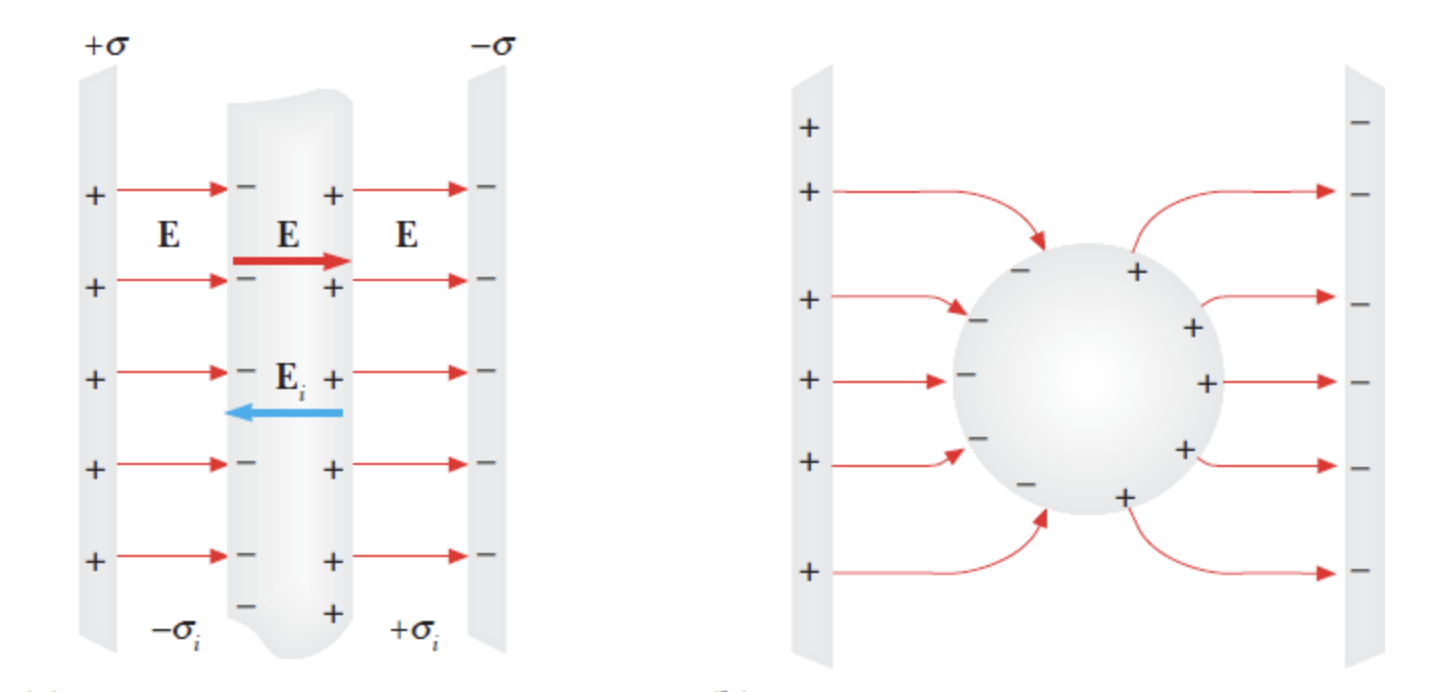
\includegraphics[width=0.8\linewidth]{figure/image30.png}
    \label{fig:chapter_7_1}
\end{figure}

Questo è il punto cruciale, perché significa che il campo delle cariche indotte tende ad annullare il campo originale. La carica continuerà a fluire finché questo annullamento non sarà completo,
e il campo risultante all'interno del conduttore sarà esattamente zero. 

\newpage

\item \emph{$\rho = 0$ all'interno del conduttore in condizioni stazionarie}. \\

Questo deriva dalle legge di Gauss in forma locale: $\nabla \cdot \mathbf{E} = \rho / \varepsilon_0$ ma se il campo è nullo all'interno allora lo sarà anche $\rho$. \\

\item \emph{I conduttori sono equipotenziali.} \\

Dati due qualsiasi punti $\mathbf{P}$ e $\mathbf{Q}$ dentro o sulla superficie del conduttore 

\begin{equation*}
    V(\mathbf{P}) - V (\mathbf{Q}) = \int_{\mathbf{P}} ^{\mathbf{Q}} \mathbf{E} \cdot d \mathbf{s} = 0 \implies V(\mathbf{P}) = V(\mathbf{Q})
\end{equation*}

\item \emph{$\mathbf{E}$ è ortogonale alla superficie e solo esterno.}\\

Dato che la superficie è equipotenziale il campo dovrà essere perpendicolare a essa e dato che all'interno deve essere nullo potrà avere componente non nulla solo all'esterno. \\

Il valore di $\mathbf{E}$ in un punto esterno molto vicino alla superficie di un conduttore si ricava applicando la legge di Gauss a un cilindro retto infinitesimo di basi $d \Sigma$ e superficie laterale di area trascurabile rispetto a $d \Sigma$, con una base contenuta all'interno del conduttore e l'altra in prossimità immediata del conduttore all'esterno. 
La carica contenuta all'interno della scatola cilindrica è $\sigma \ d\Sigma$ 

\begin{figure} [h]
    \centering
    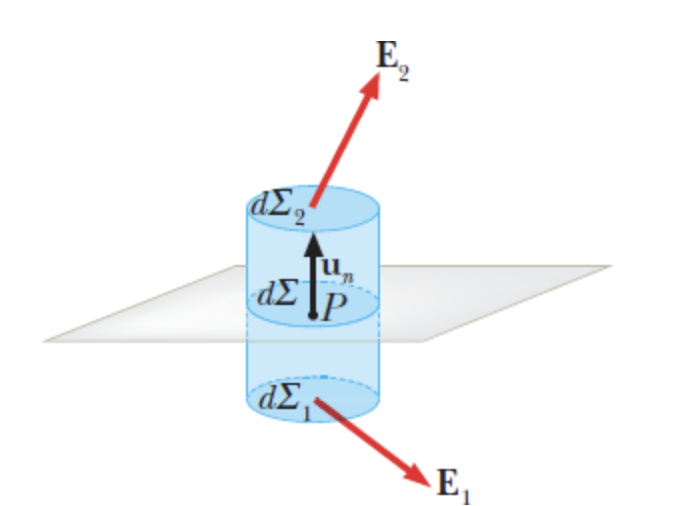
\includegraphics[width=0.5\linewidth]{figure/image31.png}
    \label{fig:chapter_7_2}
\end{figure}

allora 

\begin{equation*}
    \mathbf{E}_1 \cdot \mathbf{u}_1 \ d \Sigma + \mathbf{E}_2 \cdot \mathbf{u}_2 \ d \Sigma = (E_{2n} - E_{1n}) \ d \Sigma = \frac{\sigma \ d\Sigma}{\varepsilon_0}
\end{equation*}

Quindi si trova la relazione locale, \emph{del tutto generale}:

\begin{tcolorbox}[colback=yellow!10!white, colframe=orange!70!black, boxrule=0.8pt]
\begin{equation}
    E_{2n} - E_{1n} = \frac{\sigma}{\varepsilon_0}
\end{equation}
\end{tcolorbox}

Dato che siamo nel caso di un conduttore, $E_{1n} = 0$ in quanto interno, allora \emph{nel caso di un conduttore}

\begin{tcolorbox}[colback=yellow!10!white, colframe=orange!70!black, boxrule=0.8pt]
\begin{equation}
    \mathbf{E} = \frac{\sigma}{\varepsilon} \mathbf{u}_n 
\end{equation}
\end{tcolorbox}

\end{enumerate}

\section{Capacità di un conduttore isolato}

Supponiamo di considerare un conduttore isolato nello spazio con una distribuzione di carica superficiale $\sigma$

\begin{figure} [h]
    \centering
    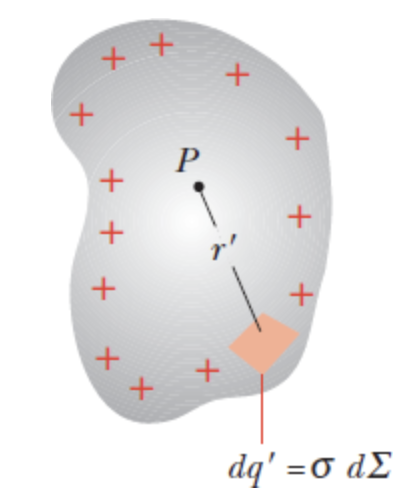
\includegraphics[width=0.30\linewidth]{figure/image32.png}
    \label{fig:chapter_7_3}
\end{figure}

allora la carica totale sarà 

\begin{equation*}
    q = \oint_{\Sigma} \sigma(x',y',z') d \Sigma
\end{equation*}

Il potenziale elettrostatico in un punto $\mathbf{P}$ qualsiasi del conduttore è dato dalla \ref{eq:potenziale_senza_condizione}

\begin{equation*}
    V = \frac{1}{4 \pi \varepsilon_0} \oint_{\Sigma} \frac{\sigma(x',y',z') d \Sigma}{r'}
\end{equation*}

Se la carica del conduttore viene portata al valore $q' = mq$ anche la densità varia localmente dello stesso fattore, $\sigma' = m \sigma$ e pure il potenziale elettrostatico del conduttore viene moltiplicato per $m$. \\

Da tali conseguenze si può dedurre che in un conduttore isolato il rapporto tra la carica elettrica e il \mkeyword{capacità del conduttore} potenziale elettrostatico non varia al variare della carica del conduttore, e tale rapporto si chiama  capacità del conduttore isolato:

\begin{tcolorbox}[colback=yellow!10!white, colframe=orange!70!black, boxrule=0.8pt]
\begin{equation}
    C = \frac{q}{V}
\end{equation}
\end{tcolorbox}

Si trova che essa dipende dalla forma e dalle dimensioni del conduttore e dal mezzo che lo circonda, in questo caso il vuoto. \\

L'unità di misura della capacità è il coulomb/volt, che prende il nome di \emph{farad}, \mkeyword{farad} simbolo $F$.

\newpage

\section{Conduttori cavi}

Consideriamo un conduttore carico che abbia nel suo interno una cavità all'interno della quale non ci siano cariche elettriche 

\begin{figure} [h]
    \centering
    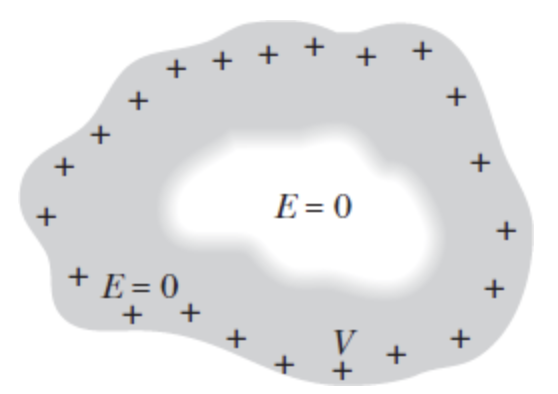
\includegraphics[width=0.4\linewidth]{figure/image33.png}
    \label{fig:chapter_7_4}
\end{figure}

Nella massa del conduttore il campo elettrostatico è nullo e pertanto il flusso è nullo è nullo attraverso qualsiasi superficie chiusa che racchiuda la cavità: segue, per la legge di Gauss, che all'interno della superficie non ci sono cariche e quindi \emph{sulle pareti della cavità la carica è nulla}.\\

Non è nemmeno possibile che sulle pareti ci sia una separazione della carica in $+q$ e $-q$ in quanto il campo elettrico è conservativo. Quindi si ha che \emph{sulle pareti della cavità non possono esserci cariche elettriche}.

\subsection{Gabbia di Faraday}

Consideriamo adesso un conduttore $C_2$ cavo, isolato e privo di carica, contenente un altro conduttore $C_1$ carico, isolato da $C_2$.

\begin{figure} [h]
    \centering
    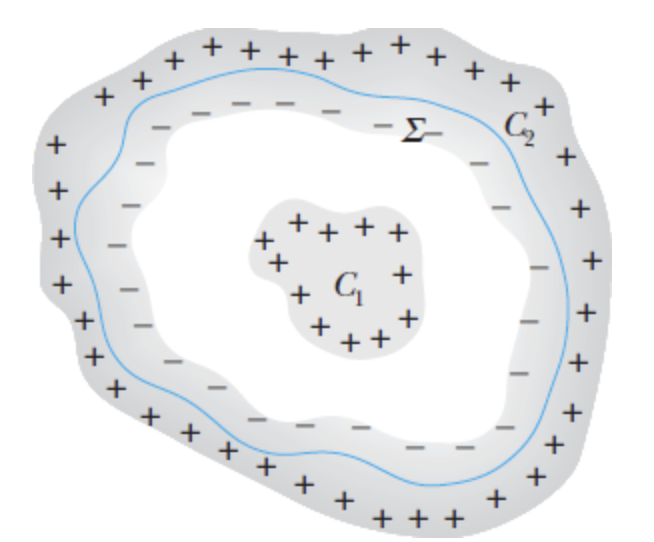
\includegraphics[width=0.4\linewidth]{figure/image34.png}
    \label{fig:chapter_7_5}
\end{figure}

In condizioni di equilibrio, se $C_1$ ha sulla sua superficie esterna una carica $q$, una carica $-q$ risulta distribuita sulla superficie interna e una carica $q$ sulla superficie esterna di $C_2$.\\

Tale fatto si spiega subito con la legge di Gauss: attraverso una superficie chiusa $\Sigma$ interna a $C_2$ e contenente la cavità il flusso di $\mathbf{E}$ è nullo in quanto è nullo il campo stesso; di conseguenza, all'interno di $\Sigma$ non c'è carica netta e se $C_1$ porta la carica $q$, sulla superficie interna di $C_2$ deve necessariamente comparire una carica $-q$. Inoltre essendo $C_2$ neutro, la distribuzione di una carica complessiva $-q$ sulla superficie interna comporta la comparsa di una carica complessiva $+q$ distribuita sulla superficie esterna.\\ 

Siamo di fronte a un fenomeno di induzione che in questo caso, essendo la carica $q$ completamente contenuta all'interno di una \mkeyword{induzione completa} cavità chiusa, si chiama induzione completa: tutte le linee di forza che partono da $C_1$ terminano su $C_2$. Dalla superficie esterna di $C_2$ partono altre linee di forza, il cui andamento in prossimità del conduttore riflette la distribuzione delle cariche sulla superficie stessa. Le due zone in cui esiste un campo non nullo sono separate da una zona in cui, in equilibrio elettrostatico, il campo elettrostatico è nullo.\\

Il campo elettrostatico all'interno della cavità è determinato dal valore di $q$, dalla posizione di $C_1$ e dalla forma geometrica delle due superfici affacciate. Però, fissato $q$ , all'esterno l'effetto è sempre lo stesso, qualunque siano forma e posizione. Infatti possiamo dire che l'informazione sulla situazione interna potrebbe passare all'esterno solo attraverso un campo elettrostatico che penetrasse nel conduttore $C_2$: ma questo non è possibile per la proprietà dei conduttori in equilibrio di avere campo elettrostatico nullo all'interno. Al limite si può portare $C_1$ a contatto con $C_2$, con il che le cariche $+q$ e $-q$ si elidono, ma all'esterno non cambia nulla: questo fatto ci fa anche capire che la distribuzione della carica $-q$ sulla faccia interna di $C_2$ è sempre tale che, sommando l'effetto della carica $q$ di $C_1$, il campo elettrostatico dovuto alle cariche nella cavità è nullo all'esterno della cavità.\\

Analogamente, se variamo la carica sulla superficie esterna oppure variamo la sua distribuzione, ad esempio avvicinando al conduttore un altro corpo carico, cambia il campo elettrostatico all'esterno, ma la distribuzione di carica sulla superficie esterna di $C_2$ è sempre tale da dare campo elettrostatico nullo all'interno di $C_2$ e quindi non può alterare il campo locale esistente nella cavità. Come osservato prima, ciò potrebbe avvenire se un campo elettrostatico penetrasse dall'esterno nella massa del conduttore, ma la possibilità è esclusa dalle proprietà di un conduttore in equilibrio.\\

Pertanto finché lo spazio interno e lo spazio esterno non sono comunicanti \emph{il conduttore cavo costituisce uno schermo elettrostatico perfetto tra spazio interno e spazio esterno.}\\

Un qualunque sistema costituito da un contenitore in materiale elettricamente conduttore (o conduttore cavo) in grado d'isolare l'ambiente interno da un qualunque campo \mkeyword{gabbia di Faraday}elettrostatico presente al suo esterno, per quanto intenso questo possa essere, prende il nome di \emph{gabbia di Faraday}.

\newpage

\section{Condensatori}

Supponiamo di avere due conduttori, il primo con carica totale $+q$ il secondo con carica totale $-q$. 

\begin{figure} [h]
    \centering
    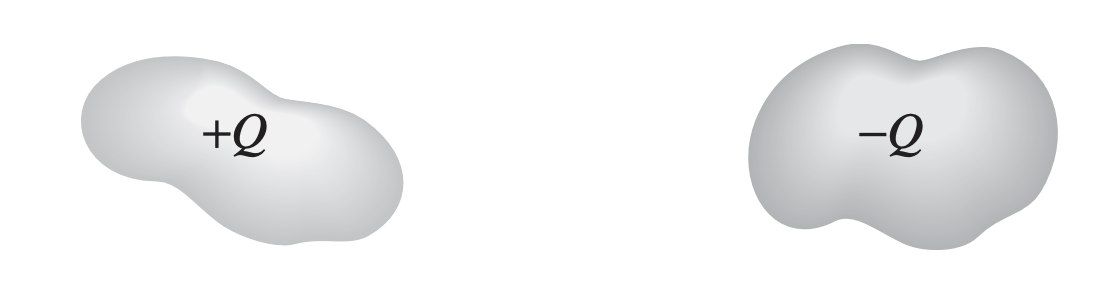
\includegraphics[width=0.65\linewidth]{figure/image35.png}
    \caption{Conduttori carichi con carica $+q$ e $-q$}
    \label{fig:chapter_7_6}
\end{figure}

Dato che il potenziale sui condensatori è costante, possiamo parlare senza ambiguità della differenza di potenziale tra i due conduttori 

\begin{equation*}
    V = V_{+} - V_{-} = \int_{-}^+ \mathbf{E} \cdot d \mathbf{s}
\end{equation*}

Non sappiamo la distribuzione delle cariche sui condensatori, tuttavia sappiamo che $\mathbf{E}$ è proporzionale a $q$. Dalla \ref{eq:campo_elettrostatico_continuo} sappiamo 

\begin{equation*}
    \mathbf{E} = \frac{1}{4 \pi \varepsilon_0} \int_{\tau} \frac{\rho}{r^2} \mathbf{u}_r \ d\tau
\end{equation*}

Quindi se raddoppiamo la carica totale sui condensatori, raddoppiamo $\rho$ e raddoppiamo anche il modulo di $\mathbf{E}$. \\

Dato che $\mathbf{E}$ è proporzionale a $q$, lo sarà anche $V$, allora andiamo a chiamare questa costante di proporzionalità \emph{capacità}. 

\begin{tcolorbox}[colback=yellow!10!white, colframe=orange!70!black, boxrule=0.8pt]
\begin{equation}
    C = \frac{q}{V}
\end{equation}
\end{tcolorbox}

Dove, in questo caso, $V$ rappresenta la \emph{differenza di potenziale tra i conduttori}. \\

Un sistema in cui tra i due \mkeyword{induzione completa} conduttori c'è induzione completa, cioè un sistema in cui tutte le linee di forza partono da un conduttore \mkeyword{condensatore} e finiscono nell'altro, prende il nome di \emph{condensatore}, mentre i due conduttori prendono il nome di armature del condensatore. \\

\newpage

Analizziamo alcuni semplici casi

\subsection{Condensatore piano} 

Un condensatore piano è formato da due piatti piani e paralleli di area $\Sigma$ posti a distanza $h$ su cui sono presenti cariche opposte $+q$ e $-q$

\begin{figure} [h]
    \centering
    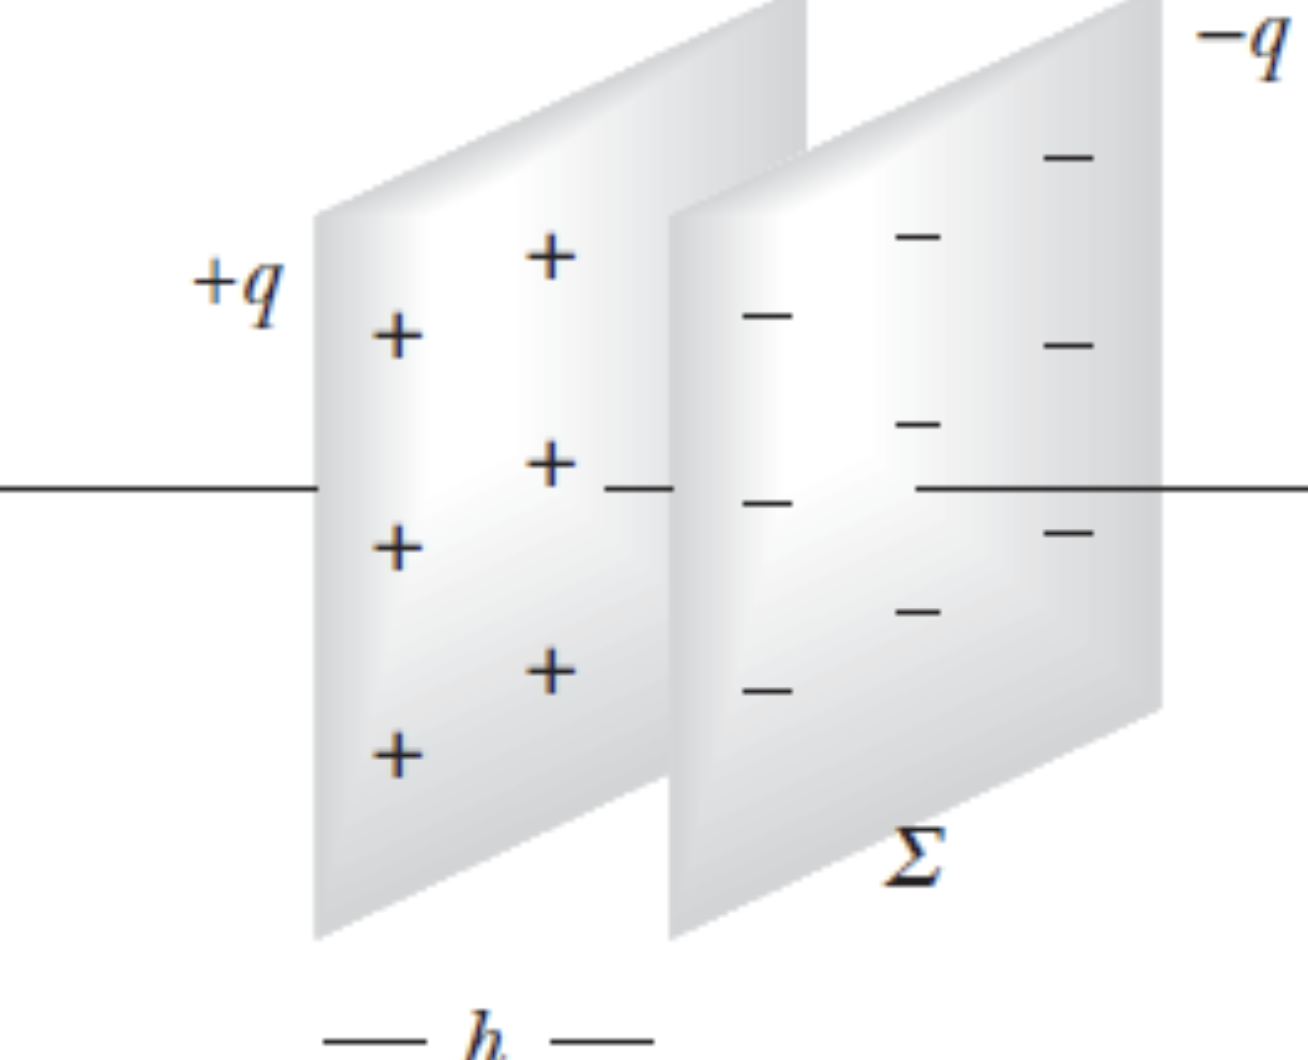
\includegraphics[width=0.4\linewidth]{figure/image36.png}
    \caption{Condensatore piano}
    \label{fig:chapter_7_7}
\end{figure}

La carica positiva $q$ è distribuita con densità uniforme $\sigma$ sull'armatura positiva e quella negativa $-q$ con densità uniforme $-\sigma$ sull'armatura negativa. Il campo interno è costante e quindi si ha

\begin{equation}
    \mathbf{E} = \frac{\sigma}{\varepsilon_0} \mathbf{u}_n \quad , \quad V_1 - V_2 = E \ h = \frac{\sigma}{\varepsilon_0} h = \frac{\sigma \Sigma}{\varepsilon_0 \Sigma} h = \frac{q}{\varepsilon_0 \Sigma} h 
\end{equation}

Si deduce quindi che la capacità di un condensatore piano è data da 

\begin{tcolorbox}[colback=yellow!10!white, colframe=orange!70!black, boxrule=0.8pt]
\begin{equation}
    C = \frac{\varepsilon_0 \Sigma}{h}
\end{equation}
\end{tcolorbox}

\subsection{Condensatore sferico}

Un condensatore sferico è un condensatore formato da due conduttori concentrici di forma sferica. In ciascun punto dell'intercapedine il campo elettrico ha simmetria radiale e un orientamento che dipende dai segni delle cariche delle due armature. \\

\begin{figure} [h]
    \centering
    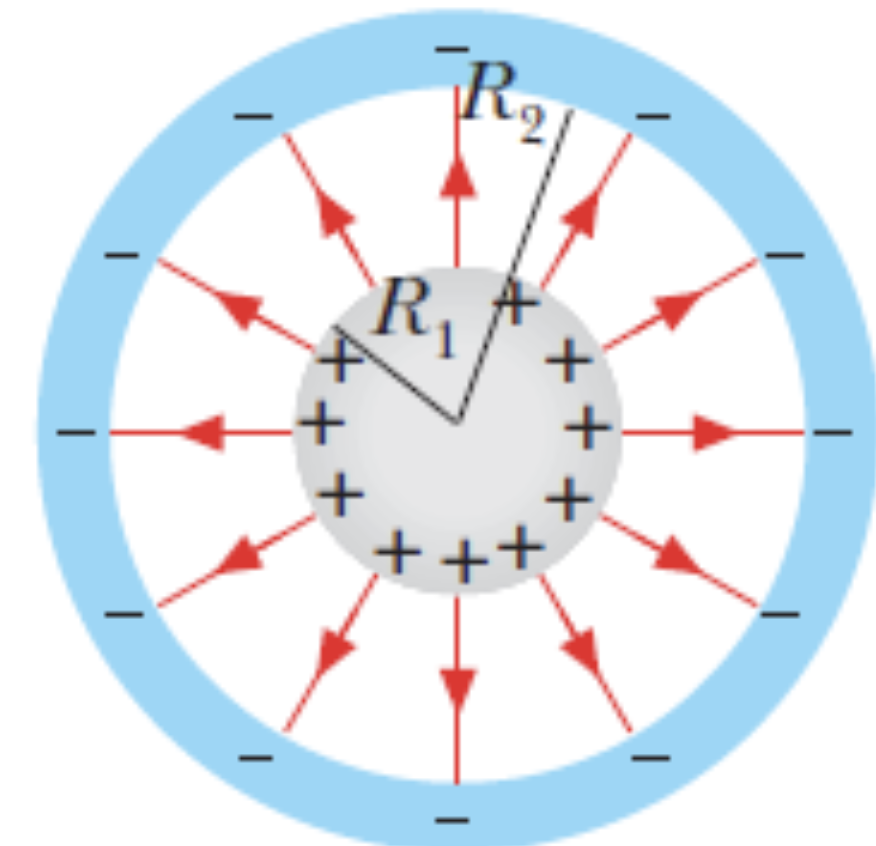
\includegraphics[width=0.4\linewidth]{figure/image37.png}
    \caption{Condensatore sferico}
    \label{fig:chapter_7_8}
\end{figure}

\' E possibile dimostrare che la capacità di questo condensatore è 

\begin{tcolorbox}[colback=yellow!10!white, colframe=orange!70!black, boxrule=0.8pt]
\begin{equation}
    C = 4 \pi \varepsilon_0 \frac{R_1 R_2}{R_2 - R_1}
\end{equation}
\end{tcolorbox}

Dove $R_1$ è il raggio della sfera interna, mentre $R_2$ quello della sfera esterna. 

\subsection{Condensatore cilindrico}

Un condensatore cilindrico è un condensatore costituito da due conduttori cilindrici coassiali. Il campo all'interno di questo condensatore è perpendicolare all'asse e radiale rispetto alla distribuzione di carica. \\

\begin{figure} [h]
    \centering
    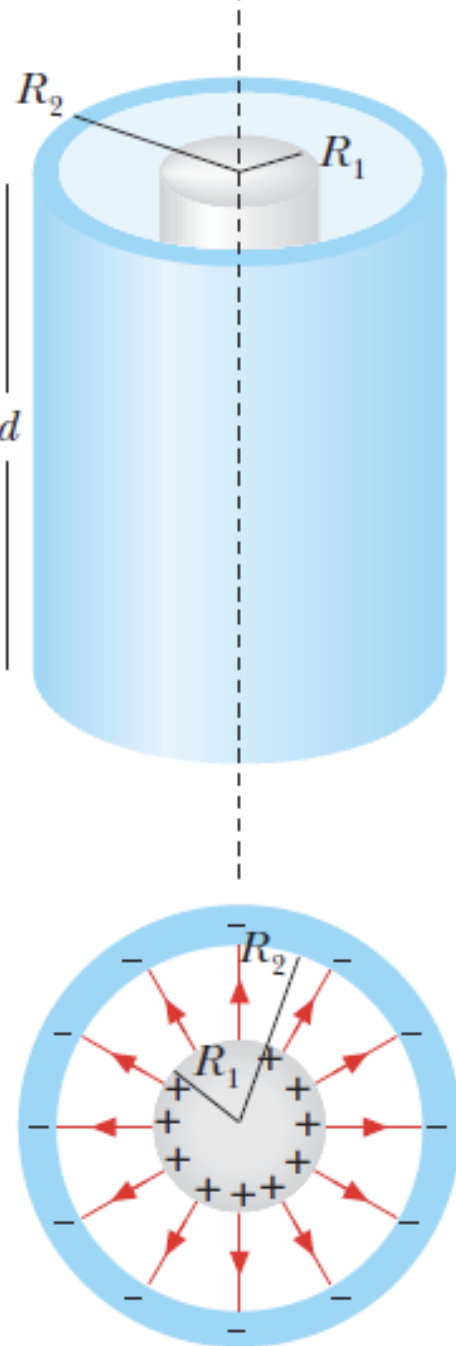
\includegraphics[width=0.25\linewidth]{figure/image38.png}
    \caption{Conduttore cilindrico}
    \label{fig:chapter_7_9}
\end{figure}

\' E facile dimostrare che la capacità di questo condensatore è 

\begin{tcolorbox}[colback=yellow!10!white, colframe=orange!70!black, boxrule=0.8pt]
\begin{equation}
    C = \frac{2 \pi \varepsilon_0 d}{\ln \left(\frac{R_2}{R_1} \right)}
\end{equation}
\end{tcolorbox}

\newpage

\section{Energia elettrostatica per i condensatori}

Il processo di carica di un condensatore, in cui si passa dalla situazione di carica zero sulle armature alla situazione $+q$, $-q$ con una differenza di potenziale $V = q/C$ tra le armature, consiste in definitiva in una separazione di cariche e richiede un determinato lavoro che, essendo il campo conservativo, dipende soltanto dallo stato iniziale e dallo stato finale, ma non dalle modalità con cui avviene il processo. \\

Per eseguire il calcolo possiamo immaginare quindi che la carica di un condensatore avvenga per processi elementari, spostando una carica $dq'$ da un'armatura all'altra, così che alla fine una carica $+q$ è stata trasferita alla seconda armatura, lasciando la prima con una carica $ - q$, e si è stabilita tra le armature la differenza di potenziale elettrostatico V; la carica totale è in ogni istante nulla.\\

Se in una fase intermedia del processo la differenza di potenziale elettrostatico tra le armature è $V'$, in quanto è già stata trasferita la carica $q' = CV'$, il lavoro fatto da un agente esterno per spostare l'ulteriore carica $dq'$ attraverso la differenza di potenziale elettrostatico $V'$ è

\begin{equation}
    dW =  V' dq' = \frac{q'}{C} dq'
\end{equation}

E quindi il lavoro complessivo per effettuare la separazione delle cariche è 

\begin{equation}
    W = \int dW = \int_0 ^q \frac{q'}{C} \ dq' = \frac{q^2}{2C}
\end{equation}

Questo lavoro, effettuato contro la forza elettrostatica che si oppone a un accumulo di cariche dello stesso segno, viene immagazzinato sotto forma di energia elettrostatica, quindi si ha 

\begin{tcolorbox}[colback=yellow!10!white, colframe=orange!70!black, boxrule=0.8pt]
\begin{equation}
    U_e = \frac{1}{2} \frac{q^2}{C} = \frac{1}{2} CV^2 = \frac{1}{2} q V
\end{equation}
\end{tcolorbox}

\section{Forza tra le armature di un condensatore}

Abbiamo trovato che l'energia elettrostatica di un condensatore dipende solo dalla geometria di quest'ultimo e dalla carica sulle armature, allora se vogliamo trovare la forza che agisce sulle armature possiamo sfruttare il fatto che 

\begin{tcolorbox}[colback=yellow!10!white, colframe=orange!70!black, boxrule=0.8pt]
\begin{equation}
    \mathbf{F} = - \nabla U_e = - \frac{q^2}{2} \nabla \left( \frac{1}{C} \right)
\end{equation}
\end{tcolorbox}

Questo vale quando \emph{la carica sulle armature è mantenuta costante}

\newpage

\subsection{Forza tra le armature di un condensatore a potenziale costante}

Invece che a carica costante il processo di spostamento dell'armatura può avvenire a differenza di potenziale elettrostatico costante: si connettono le armature ai poli di un generatore di forza elettromotrice, che è un dispositivo in grado di mantenere costante la differenza di potenziale tra esse. Di conseguenza, quando l'armatura positiva si sposta avvicinandosi all'altra armatura, V resta costante, C aumenta e quindi q deve aumentare: il processo comporta ora uno spostamento di carica da un'armatura all'altra, con spesa di lavoro. 
Pertanto quando andremo a trovare l'energia totale del sistema \emph{dovremo considerare sia l'energia dovuta alla distribuzione di carica, sia quella dovuta al generatore}.\\

La variazione di energia elettrostatica è 

\begin{equation}
    dU_e = d \left(\frac{1}{2} CV^2\right) = \frac{V^2}{2} \ dC
\end{equation}

Che è positivo. Mentre il lavoro per lo spostamento della carica $dq = V dC$ è 

\begin{equation}
    dW_{\text{gen}} = V \ dq = V^2 \ dC = - dU_{\text{gen}} 
\end{equation}

Che è negativo, in quanto è fornito a spese dell'energia interna.\\

Allora l'energia totale del sistema varia come 

\begin{equation}
    dU = dU_e + dU_{\text{gen}} = - dU_e
\end{equation}

Pertanto si ha in questo caso 

\begin{tcolorbox}[colback=yellow!10!white, colframe=orange!70!black, boxrule=0.8pt]
\begin{equation}
    \mathbf{F} = - \nabla U  = \nabla U_e = \frac{1}{2} V^2 \ \nabla C
\end{equation}
\end{tcolorbox}
